\clearpage\secrel{Classical compiler scheme}

This is classical structure used in all interpreter and compilers:
\noindent
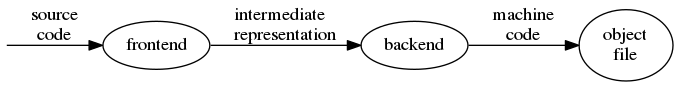
\includegraphics[width=\textwidth]{img/compiler.png}
\begin{description}[nosep]
\item[frontend] compiler part translates source code written in some programming
language syntax into IR: there are \emph{many frontends for multiple input
languages}, but \emph{single shared IR} which can be understood by any backend
\item[backend] do IR optimization and generates IR into machine code: the same
IR, and \emph{multiple target} processors
\end{description}

\clearpage\noindent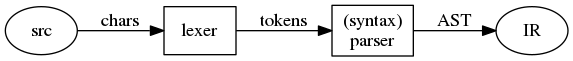
\includegraphics[width=\textwidth]{img/frontend.png} 
\begin{description}[nosep]
\item[lexer] scans input stream contains single chars of source code, and group
them into tokens: every token contains a single symbol \emph{value}, \emph{type}
tag, and location where it placed in the source code (name of a file, line
number,..). As you can see, token structure is very close to our
\verb|<type:value>| base object structure, so lexer can just return ready to use
objects.
\item[parser] eats stream of tokens and groups them into tree-like structures
according to programming language grammar. The output of parser is AST:
\term{Abstract Syntax Tree}. As \F\ has very simple sequential grammar, it does
not use syntax parser.
\end{description}

\clearpage\secrel{Lexer}
\noindent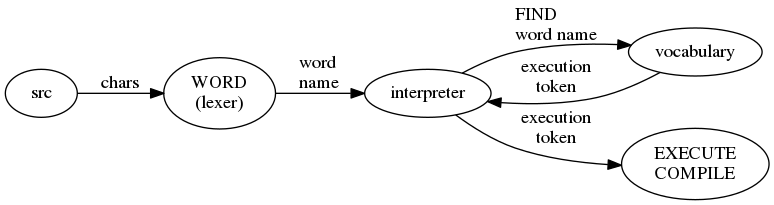
\includegraphics[width=\textwidth]{img/forthend.png} 
In classical \F\ the whole lexer is \verb|WORD| (and few words do special
lexing like \verb|\| and \verb|"| use WORD for its work). But this way has a
drawback: WORD can't distinguish word names, numbers, string and so on. If you
put 1234 in source code, \verb|WORD| returns it \emph{as string}, and
\verb|INTERPRET| must do extra work to check can it be number. If you put
\verb|" string"| you must place extra space before string content to let
interpreter first find and execute \verb|"| which will next do \verb|["] WORD|
to parse rest of string.

It is
extra easy to write classical \F\ parser in a few machine commands\note{char
reading pointer in buffer, and dumb comparing current char with spaces}, and it
is very useful in devices built on smallest microcontrollers.
But we want some \term{syntax sugar} in o\F\note{and extendable \emph{infix}
syntax in feature releases}, so we will use special parser writing library
PLY\note{and parser generators for \cpp} in place of dumb \verb|WORD|. Such
lexer will do type detection for \term{literals} (numbers, strings,..).

\clearpage
